% \Huge

\section{Information loss and potential recovery}

We studied information loss due to gravitational collapse. Our two main observational probes (CMB and Galaxy surveys) are widely separated by an era from which we have very little information, and which contains such important events as the formation of the first stars and galaxies. It is, therefore, in our interest to find ways of using the data we collect about our Universe today to recover information about the past. These reconstruction techniques have been widely used to recover information on the Baryon Acoustic Peak, but here we look to even smaller scales. Our aim was to test the limits of reconstruction as well as to look at more realistic methods and see how they perform.

In Chapter 2, we proved that some information will never be recovered. To show this, a perfect reconstruction was performed. We measured the density field at the particle positions and used the knowledge of the initial particle positions to reconstruct it. Because we do not (and cannot) measure the density field in an infinity of locations we cannot capture all of its information. This means, no reconstruction is capable of perfectly recovering the primordial density field.

Figure~\ref{fig:3.2} shows the normalized cross spectra of our reconstructed fields with the initial density field (versus the original correlation). Our reconstruction recovers plenty of  intermediate scale information and the two stay correlated to very small scales. However, on these very small scales, they do decorrelate. This information can never be recovered by reconstructing the density field. The plot shows the most amount of information that could ever be recovered from each redshift. In a way, it shows the limit of what we can ever hope to learn about the primordial density field. 

We have also shown that two of the limiting factors in reconstruction are the resolution used and the redshift. Both of these can be improved upon in practice. More and more information is destroyed with the progress of time. By detecting matter further back in time, we increase the amount of information we can recover. On the resolution side, our limitations are the size of galaxies and how many of them we can detect in a certain volume. Galaxies are also biased tracers of matter, so Galaxy Surveys might not be our best option. A very promising future probe is the Square Kilometre Array (SKA).\todo{ref} It will push both boundaries at the same time. Its goal is to detect atomic hydrogen before reionisation (using the 21cm emission). As we are looking much further back in time ($z>10$) and directly at the matter distribution, this probe will lead to incredible advancements in our knowledge of the early Universe.


After studying the limits of reconstruction, we turned our attention to more realistic methods in Chapter 3. In particular, we looked at ways of reconstruction methods within the Lagrangian framework. We first start by performing a Zel'dovich reconstruction. Particle velocities are used to calculate a displacement field within the first order approximation of Lagrangian Perturbation Theory (the Zel'dovich Approximation). As before, we calculated the density field at the particle positions and then applied the displacement field to move them back in time. The density field is also carried back in time and reconstructed. We showed that the method works very well when starting at high redshifts ($z=9$). However, when starting at late redshifts, this method creates an anti-correlation on the largest scales. This might be caused by the fact that at those redshifts ($z=0$) most particles have highly non linear velocities, however this phenomenon is not well understood. We left this Zel'dovich reconstruction as just an intermediate step because of its lack of realism (in practice we could not measure so many velocities so accurately) and its poor performance at low redshifts.

In order to improve the realism and low redshift performance of the method we investigated ways of smoothing the velocity field. We present to methods for achieving this. For the first one, we just average velocities over 1 Mpc and 10 Mpc scales respectively, and interpolate the velocities back at the particle positions. For the second one, we average velocities over smaller scales (0.5 Mpc) and apply a Gaussian filter to smooth this average velocity field over 1 Mpc and 10 Mpc scales respectively. After that, we again interpolate the velocities back at the particle positions. Finally, in both cases we use the smoothed velocities and the Zel'dovich approximation to move the particles (and the density field with them) back in time. These methods are more realistic because we are giving up the accurate and precise knowledge of all the particle velocities. Instead, we now have an average velocity field over certain scales, and this could be measured in practice. 





\section{Future Work}

\todo{talk about the fact that we assumed perfect knowledge of the final density field for realistic reconstructions}

\begin{figure}
    \centering
    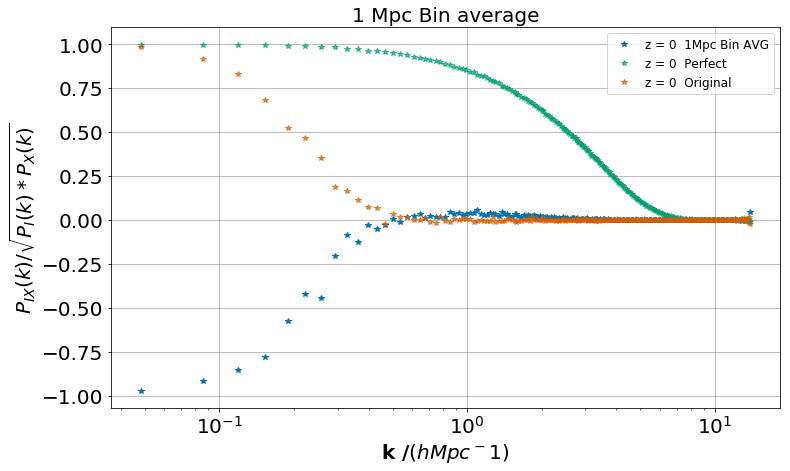
\includegraphics[width=1\columnwidth]{images/realRecon/1MpcBinAvg.png}%
    
    \caption{
        Simulation A reconstruction
    }
    
    \label{fig:12}
\end{figure}

\todo[inline]{Talk about the problems encountered and Future Work.}